% !TEX root = Entwurf_goApp.tex

\section{Client} 
	%TODO Jedes Package als subsection mit sinnvoller Bennenung und in diesen als subssubsection alle Klassen beschreiben.
	\subsection{Services}
	Im folgenden Kapitel werden alle Services die von unserer App implementiert werden beschrieben.
	Sie alle erben von der Klasse IntentService weshalb wir zusätzlich zum Konstruktor nur eine public Methode für jeden Service implementieren und zwar die Methode onHandleIntent(Intent intent).
	Weil diese Methode bei allen unserern Services je nach Intent entscheidet welche privat Methode aufgerufen wird und sonst keine weiter Funktionalität besitzt haben wir uns dazu entschieden im folgenden nicht für jeden Service auf die besagte Methode einzugehen sondern jeweils die Methoden zu beschreiben welche durch onHandleIntent(Intent intent) aufgerufen werden, da dies unserer Meinung nach eine bessere Definition der Services Klassen liefert und damit für bessere Verständlichkeit sorgt. 
	\subsubsection {LoginService}
	\subsubsection {UserService}
	\subsubsection {GroupService}
	\subsubsection {GroupSearchService}
	\subsubsection {RequestService}
	\subsubsection {RequestSearchService}
	\subsubsection {ParticipateService}
	\subsubsection {LocationService}
	\subsubsection {EventService}
	\subsubsection {GoService}
	\subsubsection {NotificationService}
	
	\subsection{Activities}
	In diesem Abschnitt werden die Activities der goApp und ihre Interaktionen mit den Services sowie die Übergänge zu anderen Activities vorgestellt.
	Da die Activities die GUI des Benutzers bilden werden hier ebenfalls die GUI-Ausschnitte aus dem Pflichtenheft, mit zusätzlichen Erweiterungen, den entsprechenden Activities durch welche sie dargestellt werden zugeordnet.  
	\subsubsection {LoginActivity}
	Die LoginActivity wird mit der App gestartet, hier kann sich ein Benutzer registrieren.
	\newline
	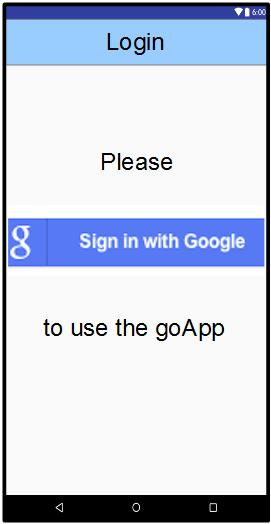
\includegraphics[width=.3\textwidth]{GUI_Login.jpg}
	\newline
	Services die von dieser Activity gestartet werden:
	\begin{itemize}
	\item LoginService
	\end{itemize}
	Von dieser Activity kann ein Benutzer zu folgenden Activities navigieren:
	\begin{itemize} 
	 \item StartActivity
	\end{itemize}
	
	\subsubsection {StartActivity}
	Die StartActivity gibt dem Benutzer eine Übersicht über alle Gruppen in denen er Mitglied ist und denen er eine Beitrittsanfrage geschickt hat.
	Außerdem kann hier der Benutzername geändert werden.
	\newline
	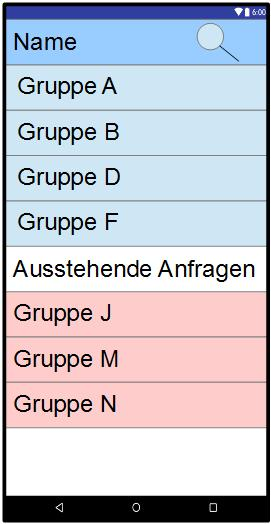
\includegraphics[width=.3\textwidth]{GUI_Start.jpg}
	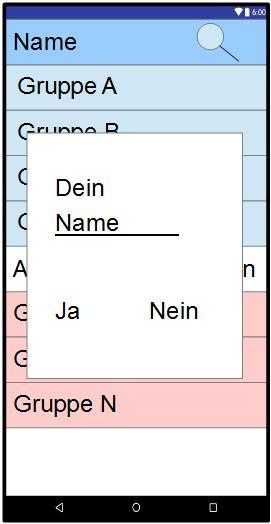
\includegraphics[width=.3\textwidth]{GUI_Start2.jpg}
	\newline
	Services die von dieser Activity gestartet werden:
	\begin{itemize}
	\item UserService
	\item GroupService
	\item GroupSearchService
	\item RequestSearchService
	\end{itemize}
	Von dieser Activity kann ein Benutzer zu folgenden Activities navigieren:
	\begin{itemize} 
	\item GroupActivity
	\item NewGroupActivity
	\end{itemize} 
	
	\subsubsection {GroupActivity}
	Die GroupActivity zeigt dem Benutzer alle anstehenden Termine einer Gruppe, bei denen er nicht abgesagt hat, an.
	\newline
	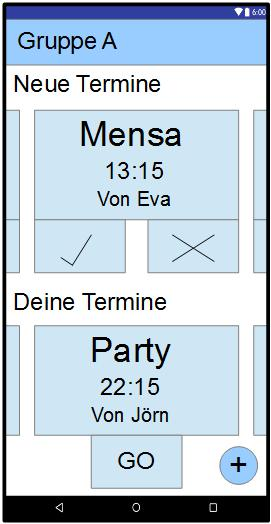
\includegraphics[width=.3\textwidth]{GUI_Group.jpg}
	\newline
	Services die von dieser Activity gestartet werden:
	\begin{itemize}
	\item EventService
	\item ParticipateService
	\item GoService
	\end{itemize}
	Von dieser Activity kann ein Benutzer zu folgenden Activities navigieren:
	\begin{itemize} 
	 \item StartActivity
	 \item GroupInfoActivity
	 \item EventActivity
	 \item NewEventActivity
	\end{itemize} 
	
	\subsubsection {GroupInfoActivity}
	Die GroupInfoActivity zeigt einem Mitglied der Gruppe deren Mitglieder an und bietet die Möglichkeit aus der Gruppe auszutreten. Der Gruppengründer sieht zusätzliche Beitrittsanfragen an die Gruppe und kann diese bearbeiten, er kann auch Mitglieder entfernen und die Gruppe löschen.
	\newline
	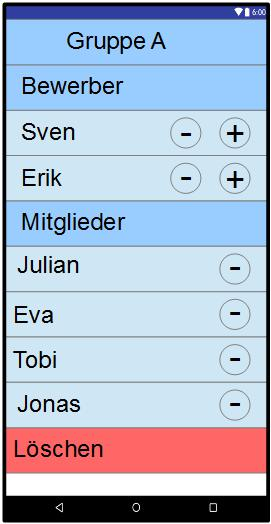
\includegraphics[width=.3\textwidth]{GUI_GruppeInfoGruender.jpg}
	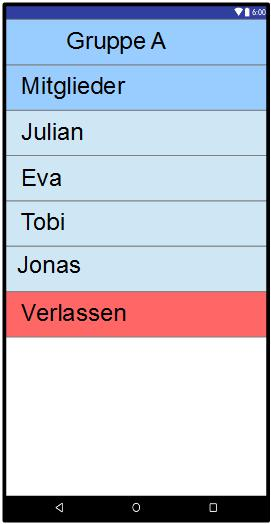
\includegraphics[width=.3\textwidth]{GUI_GruppeInfoNormal.jpg}
	\newline
	Services die von dieser Activity gestartet werden:
	\begin{itemize}
	\item GroupService
	\item RequestService
	\item RequestSearchService
	\end{itemize}
	Von dieser Activity kann ein Benutzer zu folgenden Activities navigieren:
	\begin{itemize} 
	 \item GroupActivity
	 \end{itemize}
	 
	\subsubsection {NewGroupActivity}
	Die NewGroupActivity ermöglicht es einem Benutzer nach Gruppen zu suchen um diesen Beitrittsanfragen zu schicken und neue Gruppen zu erstellen.
	\newline
	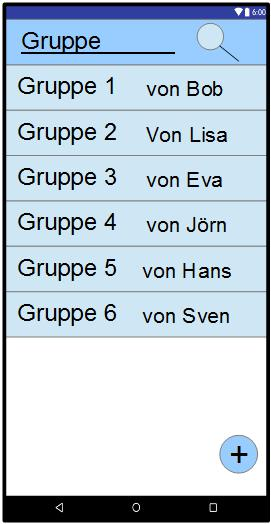
\includegraphics[width=.3\textwidth]{GUI_NeueGruppe.jpg}
	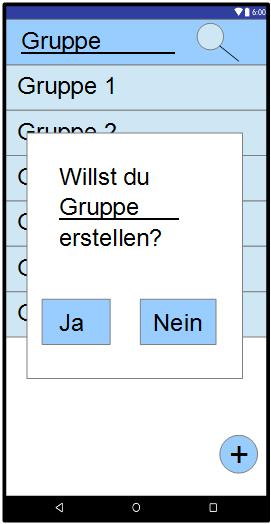
\includegraphics[width=.3\textwidth]{GUI_GruppeNeuBest.jpg}
	\newline
	Services die von dieser Activity gestartet werden:
	\begin{itemize}
	\item GroupService
	\item GroupSearchService
	\item RequestService
	\end{itemize}
	Von dieser Activity kann ein Benutzer zu folgenden Activities navigieren:
	\begin{itemize} 
	 \item StartActivity
	 \item GroupActivity
	 \end{itemize}
	 
	\subsubsection {EventActivity}
	Die EventActivity lässt einen Benutzer alle Informationen zu einem Termin einsehen und bindet eine dynamische Karte ein.
	\newline
	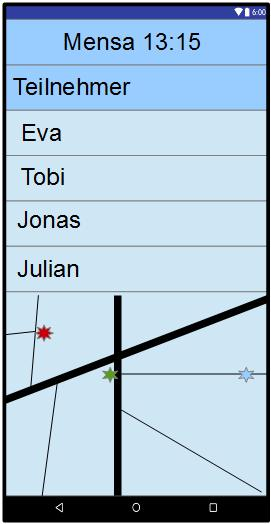
\includegraphics[width=.3\textwidth]{GUI_Termin.jpg}
	\newline
	Von dieser Activity kann ein Benutzer zu folgenden Activities navigieren:
	\begin{itemize} 
	 \item GroupActivity 
	 \end{itemize}
	 
	\subsubsection {NewEventActivity}
	Die NewEventActivity lässt einen Benutzer ein neues Event erstellen.
	\newline
	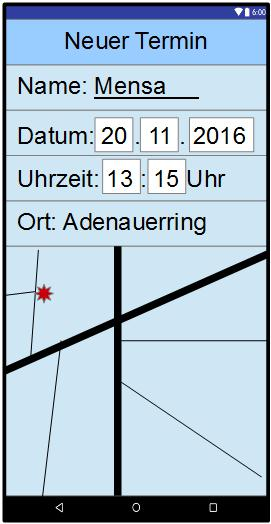
\includegraphics[width=0.3\textwidth]{GUI_NeuerTermin.jpg}
	\newline
	Services die von dieser Activity gestartet werden:
	\begin{itemize}
	\item EventService
	\end{itemize}
	Von dieser Activity kann ein Benutzer zu folgenden Activities navigieren:
	\begin{itemize} 
	 \item GroupActivity
	 \end{itemize}
	
	\subsection{Model}
	%TODO bei Datenbank auf Clienten die entsprechenden Packages eintragen.
	\newpage